\chapter{RGD Family of Models}

\section{RGD model}

This section briefly summarizes the workflow of RGB model written in MATLAB. More detail description can be seen in \referencename~\cite{ref:zhang2020a}.  This code is for symmetric full blade which is defined as D1 bit in the paper.  The code calculates coupled PDE and ODE by solving the matrix
\begin{equation}\label{matrix}
  \bm{Adx} + \bm{BX} = \bm{Q}
\end{equation}
where $\bm{dx}$ and $\bm{X}$ are defined as follow:

\noindent\begin{minipage}{.5\linewidth}
\begin{equation}
\bm{x}=
\begin{bmatrix}
\dot{u} \\
u \\
\psi \\
\dot{\psi} \\
a_1\ \\
\vdots \\
a_N \\
\end{bmatrix}
\end{equation}
\end{minipage}%
\begin{minipage}{.5\linewidth}
\begin{equation}
\bm{dx}=
\begin{bmatrix}
\ddot{u} \\
\dot{u} \\
\dot{\psi} \\
\ddot{\psi} \\
\dot{a_1}\ \\
\vdots \\
\dot{a_N} \\
\end{bmatrix}
\end{equation}
\end{minipage} \\

The bit trajectory function which is $\overline{h}(\tau, \theta$) is introduced and PDE can be derived from equation:
\begin{equation}\label{PDE}
\frac{\partial \overline{h}}{\partial \tau} + (w_0 + \dot{\psi})\frac{\partial \overline{h}}{\partial \theta}-v_0 = 0
\end{equation}

Equation (\ref{PDE}) is solved by Galerkin-method which approximates $\overline{h}(\tau, \theta$) by using base functions $a_1, a_2, ..., a_N$ (N=25 as default), where $\tau$ is scaled time and $\theta$ is rotation angle of the bit blade. The base functions can be obtained by minimizing the residual which are shown below (please note that all the derivations are for D1-bit):

\begin{equation}\label{GM}
\begin{split}
R &= \left(\frac{n \theta}{2 \pi}-1\right)\dot{u}_b + \frac{n \theta}{2 \pi}\dot{a}_1 + \sum_{k=1}^{N-1}\dot{a}_{k+1}sin\left(\frac{nk\theta}{2}\right) \\ + &(w_0 + \dot{\psi}_0)\left[u_b\frac{n}{2\pi}+a_1\frac{n}{2\pi} + \sum_{k=1}^{N-1}\frac{a_{k+1}nk}{2}cos\left(\frac{nk\theta}{2}\right)\right]
\end{split}
\end{equation}

where n is the number of bit blade. In the paper the blade number is divided to $n_i$, and $n_o$ that are number of inner blades and outer blades, respectively. However, the codes runs for D1 bit and it contains n instead of $n_i and n_o$.

Minimizing $R(\theta, \tau)$ can be acheived by making it orthogonal to the base functions over the domain $\theta \in \left[0, \frac{2\pi}{n_i}\right]$, which results in:

\begin{equation}\label{GM1}
 \int_{0}^{\frac{2\pi}{n}}R(\theta,\tau)\frac{n\theta}{2\pi}d\theta = 0
\end{equation}

and

\begin{equation}\label{GM2}
 \int_{0}^{\frac{2\pi}{n}}R(\theta, \tau)sin\left(\frac{n_im\theta}{2}\right)d\theta=0, m= 1,....,N-1
\end{equation}
where N is the number of Galerkin base functions.

Equation (\ref{GM1})-(\ref{GM2}) represent a system of N first order equations for $a_i, i=1,2,...,N$ that is

\begin{equation}\label{Norder}
  \dot{a}_i = \Phi_i(\dot{u}, u, a_1, ..., a_N), i=1,...,N.
\end{equation}

Which is coupled with the equation of motion (governing equation) which are:

\begin{equation}\label{GE1}
  \varpi-\varpi_0 = n(\delta_n - \lambda(g(\nu)) - \frac{2\pi v}{w_0}
\end{equation}

\begin{equation}\label{GE2}
  \Gamma-\Gamma_0 = n(\delta_n -\beta \lambda(g(\nu)) - \frac{2\pi v}{w_0}
\end{equation}

where $\delta_n$ is given as:

\begin{equation}\label{deltan1}
  \delta_n = \overline{h}\left(\frac{2\pi}{n}, n\right) + u(\tau)
\end{equation}

$\varpi$, $\Gamma$ represent scaled WOB, TOB, respectively,  $\beta$ is number characterizing bit/rock interaction (generally less than 1). v and w are the scaled axial and angular velocity, respectively that are

\begin{equation}\label{scaled_axial_ve}
  v = v_0 + \dot{u}
\end{equation}
\begin{equation}\label{scaled_angular_vel}
  w = w_0 + \dot{\psi}
\end{equation}

So far we have N+2 equations with N+4 unknowns ($u, \dot(u), \psi, \dot(\psi), a_1, ..., a_N$). and two additional equations are obtained from relationship below:

\begin{equation}\label{axial_dis_vel}
  \dot{u} = \frac{\partial u}{\partial \tau}
\end{equation}
\begin{equation}\label{angular_dis_vel}
  \dot{\psi} = \frac{\partial \psi}{\partial \tau}
\end{equation}

Finally we obtained N+4 equations for the same number of unknowns and represent as linear from of $\bm{Adx} + \bm{BX} = Q$. and solve the equation for given time interval. However, the discontinuity should be investigated every time step which affects the boundary condition from rock-bit interaction. The model classifies the discontinuity to three which are 1) normal drilling, 2) axial stick, and 3) bit bonce. Below summarizes the conditions for each mode:

\begin{equation}\label{drillingmodes}
  \begin{cases}
    Normal\,drilling, & \mbox{if $\delta_n > 0, w > 0$, and $v > 0$ }  \\
    Axial\, stick, & \mbox{if $\delta_n >0, w > 0$, and $v = 0$ } \\
    Bit\,bounce, & \mbox{if $\delta_n = 0$, and $w > 0$}
  \end{cases}
\end{equation}

\section{Normal drilling}
Normal drilling mode simplifies the equations (\ref{GE1}), and (\ref{GE2}) since g($\nu$) = 0 which can be represented as:

\begin{equation}\label{GE1_normaldrilling}
  \varpi-\varpi_0 = n\left(\delta_n - \frac{2\pi v}{w_0}\right)
\end{equation}

\begin{equation}\label{GE2_normaldrilling}
  \Gamma-\Gamma_0 = n\left(\delta_n - \frac{2\pi v}{w_0}\right)
\end{equation}

Also, the depth of cut (\ref{deltan1}) is reduced to:

\begin{equation}\label{deltan_normaldrilling}
  \delta_n = a_1 + u(\tau)
\end{equation}

Afterwards, equation (\ref{matrix}) can be solved with reduced equations from equations (\ref{GE1_normaldrilling}) - (\ref{deltan_normaldrilling})

\newpage
\section{Extended RGD model (Zhang and Detournay, 2022)}


This section summarizes the paper from Zhang and Detournay 2022, which is an extension of RGD model. The proposed model is a multi-degrees of freedom (MDOF) model of a rotary drilling system simulating axial-torsional self-excited vibrations induced by the bit/rock interactions. \figurename~\ref{model_develop_figure} illustrates the development of the RGD model.

\begin{figure}[ht]
  \centering
  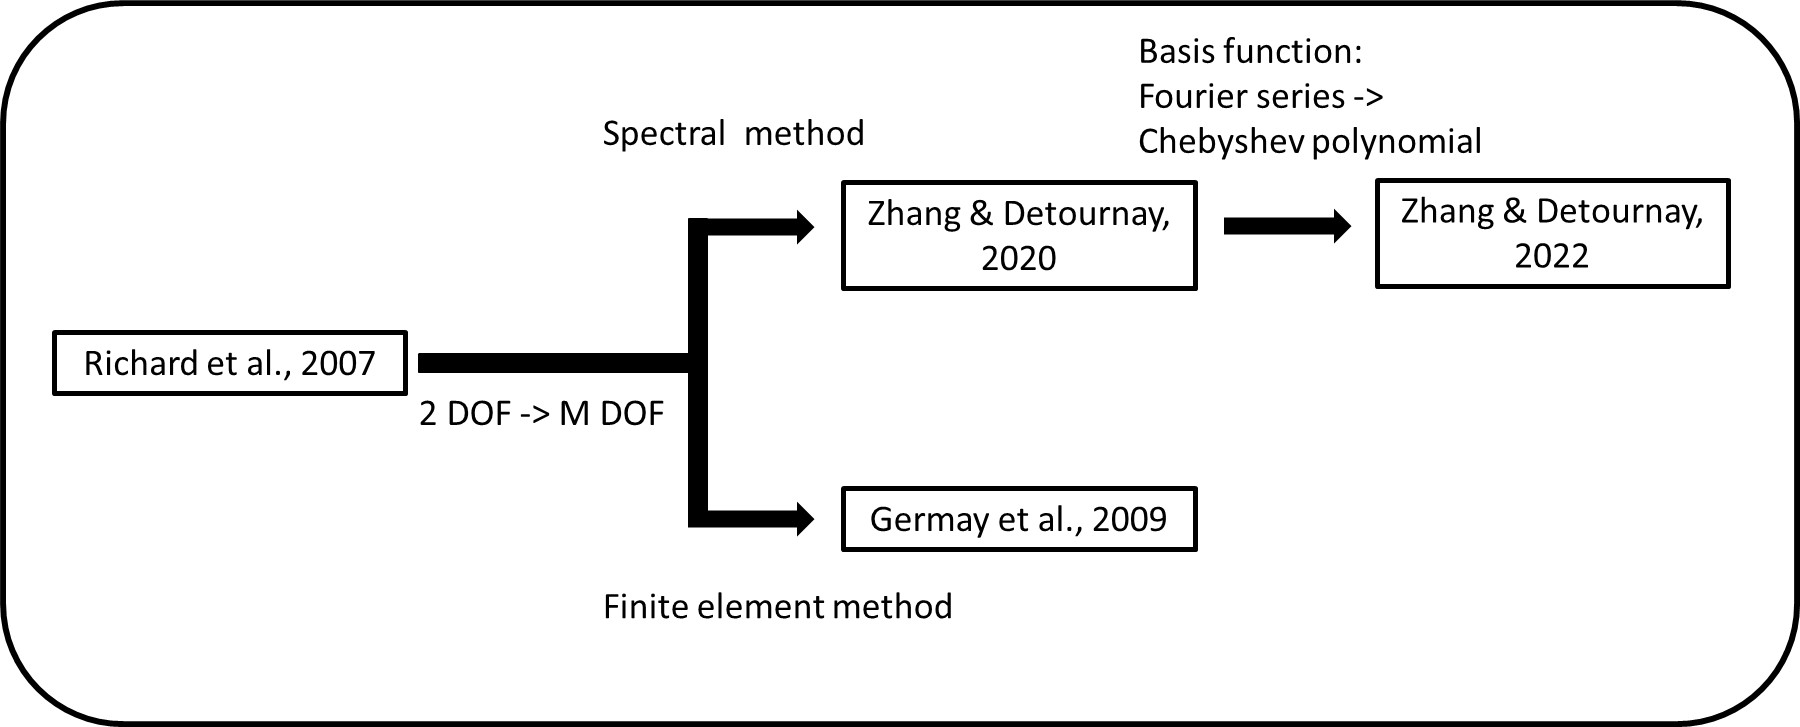
\includegraphics[width=5in]{ModelDevelop}
  \caption[RGD model development]{RGD model development.}\label{model_develop_figure}
\end{figure}

The model represents the drillstring with multiple damped axial and torsional oscillators and the bit with symmetrically arranged blades. The schematic of MDOF model of the drillstring is shown in Figure \ref{MDOF_illustration}. The model takes into account damping and
different properties of drill pipe and BHA

\begin{figure}[ht]
  \centering
  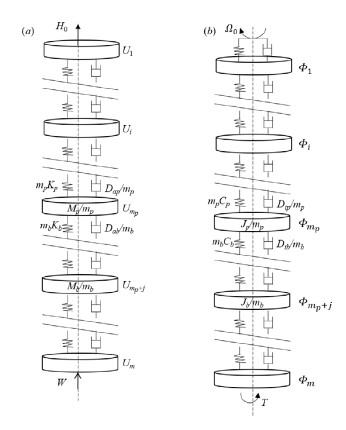
\includegraphics[height=3in]{MDOF_illustration}
  \caption[Schematic of the MDOF model of the drillstring]{Schematic of the MDOF model of the drillstring. a) axial, b) torsional.}\label{MDOF_illustration}
\end{figure}

The following assumptions are made: 1) The borehole is vertical, 2) Lateral vibration of the drillstring are neglected, 3) axial and torsional damping are proportional to the length of drill pipes and BHA, 4) constant hook load and rotary speed from surface (surface boundary conditions). Additionally, the discontinuity of the boundary condition at the bit-rock interface is modeled by
five different regimes classified based on axial, angular velocities, and depth-of-cut, namely, 1) normal drilling, 2) axial stick, 3) loss of contact, 4) torsional stick, 5) backward rotation

The system equations (PDE-ODE coupled) are established from equation of motions (axial and torsional), and bit trajectory function, which is defined to project depth of cut from the angular displacement of the bit. Then,
The PDE-ODE coupled system is numerically solved by discretizing the PDE-ODEs into ODEs. In this study, spectral method with Chebyshev polynomial is applied rather than finite element (FEM) or finite different method (FDM). Spectral method achieved high accuracy for a given number of basis functions and also converged faster compared to other numerical methods. (this is valid with simple geometry). \\

\noindent Some of the results and potential of the model are summarized below.
\begin{bulletedlist}
  \item Modeling the vibrations of entire drillstring (not only the bit).
  \item Possible to conduct frequency analysis since it is multi-degrees of freedom model (\figurename~\ref{StickslipExample}).
  \item It can simulate axial and torsional vibrations including stick-slip event (\figurename~\ref{Axial_torsional_vibration_example}).
  \item Mode analysis can be done by computing the eigenvalues of the linearized system of equation.
  \item Computationally efficient compared to FEM assuming geometrically simple structure.
\end{bulletedlist}

\begin{figure}[ht]
  \centering
  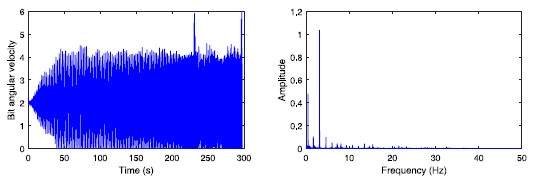
\includegraphics[width=6in]{StickslipExample}
  \caption[Simulation results of bit angular velocity and its frequency spectrum]{Simulation results of bit angular velocity and its frequency spectrum. The result shows the stick-slip occupance due to self-excited torsional vibration}\label{StickslipExample}
\end{figure}

\newpage

\begin{figure}[ht]
  \centering
  \includegraphics[height=5in]{Axial_torsional_vibration_example}
  \caption[Simulation results showing axial and angular velocity with scaled time]{Simulation results showing axial and angular velocity with scaled time. a) stable regime, b) slow regime of instability, c) fast regime of instability.}\label{Axial_torsional_vibration_example}
\end{figure}

\noindent The following are key questions or points that should be addressed for the model selection.
\begin{bulletedlist}
  \item Can we model deviated or horizontal well?
  \item Geometrical nonlinearity in drillstring (for deviated well).
  \item Can we take int to account the effect of contact point?
  \item No lateral vibration - only modeling axial, torsional motion.
  \item Decoupling of axial and torsional vibration. this can be important when it comes to 3D model (i.e., whirling effect).
  \item Current code provided is 2 DOF model.
\end{bulletedlist} 

\newpage
\chapter{Aarsnes-Shor model}

\section{Aasnes-Shor model}

The proposed model applies the distributed model of the drillsring with the Coulomb friction given as distributed source term. Most of the previous studies explained the stick-slip behaviour from bit-rock interaction \referencename~\cite{ref:germay2009a, ref:richard2007a, ref:zhang2020a}. Therefore theses models could not validate the stick-slip behavior while off bottom state (i.e., back reaming). The proposed model simulates the torsional stick-slip by take in to account Coulomb-type friction throughout the drillstring. The effect of the distributed, along-string, Coulomb friction becomes prominent of torsional drill string dynamics in wellbores with high-inclination laters. The model was validated with field data from rotational startups, off bottom rotation (without any axial movement), after connection.\\

\noindent Assumptions of the model are listed below:
\begin{bulletedlist}
    \item No bit-rock interaction
    \item No lateral and axial motion
    \item the effects of cuttings distribution on the friction is homogeneous
    \item The transition from static to dynamic coulomb friction is modeled as a jump
\end{bulletedlist}


\noindent Mathematical procedure is summarized below (follows the code flow provided):

The model is based on the euqations of angular motion, here named wave equation, which is:
\begin{equation}\label{AS-motion}
  J\rho\frac{\partial w(t,x)}{\partial t} + \frac{\partial \tau (t,x)}{\partial x} = S(w,x)
\end{equation}
where J is polar moment of inertia and $\rho$ is material density, $w(t,x)$ is angular velocity, $\tau(t,x)$ is torque, and S is the source term which can be represented as:
\begin{equation}\label{AS-sourceterm}
  S(w,x) = -k_t \rho J w(t,x) - \mathcal{F}(w,x)
\end{equation}
where $k_t$ is damping constant which is viscous shear stresses from drilling mud and cuttings bed, and $\mathcal{F}(w,x)$ is Coulomb friction between the drill string and the borehole. 
The 
The partial wave equation is transformed into their Riemann invariants and it is solved by first order upwind scheme. The Riemann invariants are defined as:
\begin{equation}\label{AS-Riemann}
  \alpha = w + \frac{c_t}{JG}\tau, \quad \beta=w-\frac{c_t}{JG}\tau
\end{equation}
where $c_t = \sqrt{\frac{\rho}{J}}$ is the velocity of the torsional wave. and the variable $\alpha, \beta$ satisfies the PDE system below:
\begin{equation}\label{AS-Riemann_alpha}
  \frac{\partial \alpha}{\partial t} + c_t\frac{\partial \alpha}{\partial x} = -\mathcal{S}
\end{equation}
\begin{equation}\label{AS-Riemann_alpha}
  \frac{\partial \beta}{\partial t} - c_t\frac{\partial \beta}{\partial x} = -\mathcal{S}
\end{equation}

where the source term $\mathcal{S}$ is
\begin{equation}\label{AS-source}
  \mathcal{S} = \frac{S}{J \rho} j= k_t(\alpha + \beta) + \frac{1}{J \rho} \mathcal{F}
\end{equation}
The boundary conditions are given as:
\begin{equation}\label{AS-BC}
  w_{p,top} = w_{TD} \quad \tau_{c,bottom} = \tau_{bit}
\end{equation}
where subscript p, c represents drill pipe and drill collar.
Additionally, the conditions at the drill pipe - drill collar interface are imposed:
\begin{equation}\label{AS-interface}
  w_{p,interface} = w_{c,interface}, \quad \tau_{p,interface} = \tau_{c,interface}
\end{equation}
\equationname~\ref{AS-BC} and \ref{AS-interface} in Riemann invariants can be written as:
\begin{equation}\label{AS-riemannBC}
  \alpha_{p,top} = -\beta_{p,top} + 2*w_{TD}, \quad \beta_{c,bottom} = \alpha_{c,top} - 2\tau_{bit} \frac{c_t}{J_c G_c}
\end{equation}
**Have to check the equation above... This boundary condition seems to take into account the torque from the bit**
\begin{equation}\label{AS-riemanninterface}
\begin{split}
    & \beta_{p,bottom} = \frac{1}{1+\overline{Z}}\left(\alpha_{p,bottom}(1-\overline{Z}) + 2\overline{Z}\beta_{c,top} \right) \\
    & \alpha_{c,top} = \frac{1}{1+\overline{Z}}\left(2*\alpha_{p,bottom} - \beta_{c,top}(1-\overline{Z})\right)
\end{split}
\end{equation}
where $\overline{Z}$is the relative magnitude of the impedance (assuming same $c_t$ for drill pipe and collar - ** need to be checked** ):
\begin{equation}\label{AS_Zbar}
  \overline{Z} = \frac{J_c G_c}{J_p G_p}
\end{equation}

\figurename~\ref{AS_discretizeDS} illustrates the schematic view of the discretized drillstring with boundary conditions, and interface conditions in terms of Riemann invariants. The boundary conditions at the top and bottom of the drillsring are applied to $\alpha$, and $\beta$, respectively. However, since the two variables are coupled by interface conditions, the PDE can be solved. 
The PDE is solved from upwind scheme according to:

\newpage
\begin{figure}[ht]
  \centering
  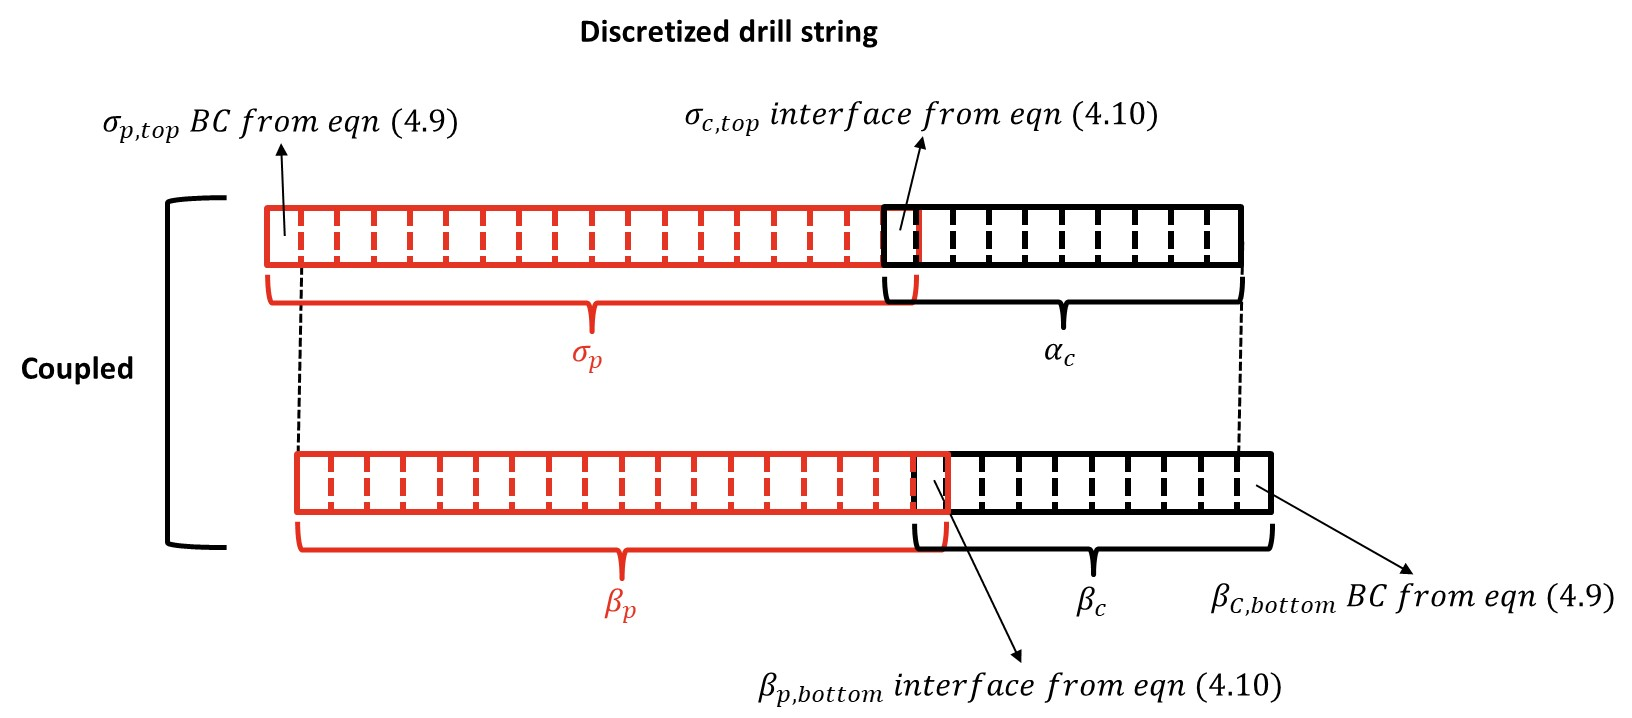
\includegraphics[width=6in]{AS_discretizedDS}
  \caption[Schematic of discretized drillstring and boundary conditions]{Schematic of discretized drillstring, boundary conditions, and interface conditions based on Riemann invariants $\alpha$, and $\beta$.}\label{AS_discretizeDS}
\end{figure}

